%Introduction

\section{Introduction}
\justify The High voltage electrical instruments have a unique problem of failure due to the breakdown of insulation strength. As the insulation of live electrical conductor fails, the purpose and function of electrical instrument stop leading toward the failure of the system. Because of partial discharge of Current Transformers will give rise to the failure of product resulting in the disruption in the supply of the system. Measurement of Partial discharge will help in predicting failure of insulation strength of Current Transformers, and corrective actions can be planned to avoid the failure of Instrument. Current transformers are used for measurement and protection application. The current transformers in electrical system step down the primary current to 5 A or 1 A. \setlength{\parskip}{1em}

Current ~Transformers ~are ~designed ~considering ~accuracy ~and ~protection requirements and current carrying capacity of the system, best insulating materials, cores and other materials are used \setlength{\parskip}{0em} \cite{crichton1989partial}.

\subsection{Partial discharge phenomenon}
Partial discharges are discharges of electrical energy in insulation material in high voltage electrical equipment's in the form small sparks. Electrical breakdown occurs after failure of insulation material due to partial discharge effect. The capacity and capability of insulation media and analysis of Partial discharge help in knowing insulation strength of instrument. The partial discharge of high voltage electrical instruments can be measured off line or Online. Measurements of partial discharge help in knowing healthy status of instruments current transformers. The electric dielectric strength and tensile strength of material decide the capability of current flow and electrical discharge during operating conditions. The insulating materials used in high voltage instruments are oil, SF\textsubscript{6} gas or mica and for low voltages epoxy, polyesters are used as insulating material. The breakdown current in the system can be known by measuring partial discharge \cite{van1994physics, danikas1998some, paithankar1997can}.\setlength{\parskip}{1em}

High voltage electrical equipment undergoes various kind of stresses during operating conditions. The electrical conducting material has thermal, chemical, mechanical stress. The reliability of electrical instrument depends upon susceptibility to these stress.

The partial discharge will cause stresses, and it will make insulation strength of oil, insulating material used in a conductive winding. The weakening or failure of insulating material will lead to generate small voids in the instrument. This will initiate the process of partial discharge and will lead to failure of an instrument. Partial discharge gives the indication of instrument failure and warning of instrument breakdown. The electric arc formed in partial discharge will reduce the dielectric strength of the material and will also have an effect on mechanical properties. The insulation of winding will become weak, and hence there will be breakdown and possibility of a fault in the system. Partial discharges in a current transformer give the indication futuristic failure. Thus, partial discharge is the tool to identify insulating strength of Current transformers \setlength{\parskip}{0em} \cite{kolev1998partial}.

\subsubsection{Partial discharge phenomenon in high voltage current transformers}
The conductive live part of electrical instruments is protected by insulation strength of the material used. The insulation failure is due to either aging effect of insulation or failure of dielectric strength of the material. If we know the reasons of insulation failure, the corrective action will have improvement and avoid re occurrence of a failure.\setlength{\parskip}{1em}

The main application of current transformers is protection through relays or for measurement through meters.

The application of Current Transformers is to maintain accuracy in measurements and can be achieved by controlling manufacturing processes and best quality of raw material. The measurement of Partial Discharge helps in knowing the potential reasons for equipment failure \cite{ren2006simulation}.

The electrical stresses in the insulation of high voltages current transformers give discharges of energy. This phenomenon is called partial discharge which will discharge energy continuously but will not lead to the failure of equipment. If this discharge is continued with high strength will lead to weaken insulation strength. The electrical stress increases, after certain limit it will lead to complete failure of the instrument. The existence of voids in solid or liquid insulating media will also reduce the insulating strength of dielectric media. This partial discharge phenomenon can occur in this void. When the electrical stresses in the void are more, will lead to breakdown and discharge phenomenon will occur \cite{kolev1999approach}.

Partial discharge is defined as electric charge Coulomb C. Since this charge is very minor defined in terms of pico. Unit of partial discharge is pico coulombs pC.

The partial discharge can be controlled by major actions during the manufacturing process in controlled environmental conditions. Avoid the voids in paper and oil insulating material. Use of a quality insulating material having high dielectric insulation \setlength{\parskip}{0em}\cite{satish1994artificial}.

\begin{figure}[h!]
    \centering
    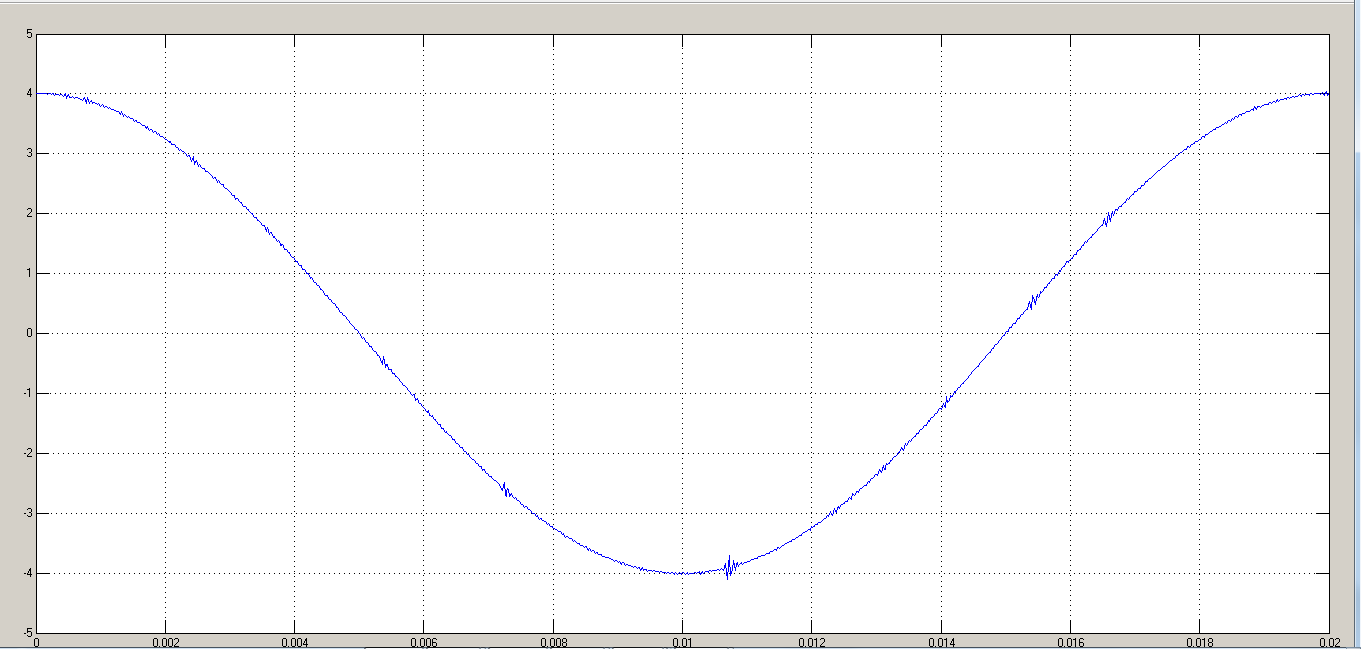
\includegraphics[width=\textwidth]{InputACSineWave145kV}
    \caption{Input AC Sine Wave 145 kV}
    \label{fig:Input AC Sine Wave 145 kV}
\end{figure}

\begin{figure}[h!]
    \centering
    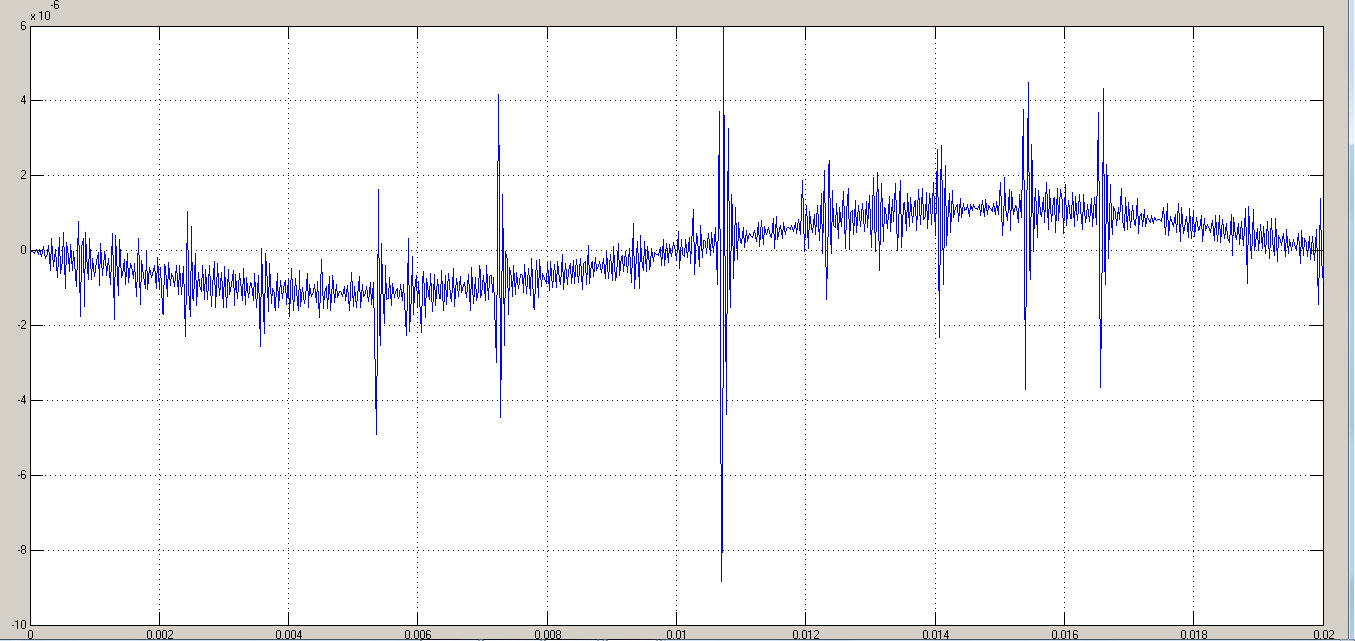
\includegraphics[width=\textwidth]{OutputACSineWave145kVwithPartialDischargepulses}
    \caption{Output AC Sine Wave 145 kV with Partial Discharge Pulses}
    \label{fig:Output AC Sine Wave 145 kV with Partial Discharge Pulses}
\end{figure}

\begin{figure}[h!]
    \centering
    
\includegraphics[width=\textwidth]{TreeingProcessduetoPartialDischarge}
    \caption{Treeing Process  due to Partial Discharge}
    \label{fig:Treeing Process  due to Partial Discharge}
\end{figure}

\begin{figure}[h!]
    \centering
    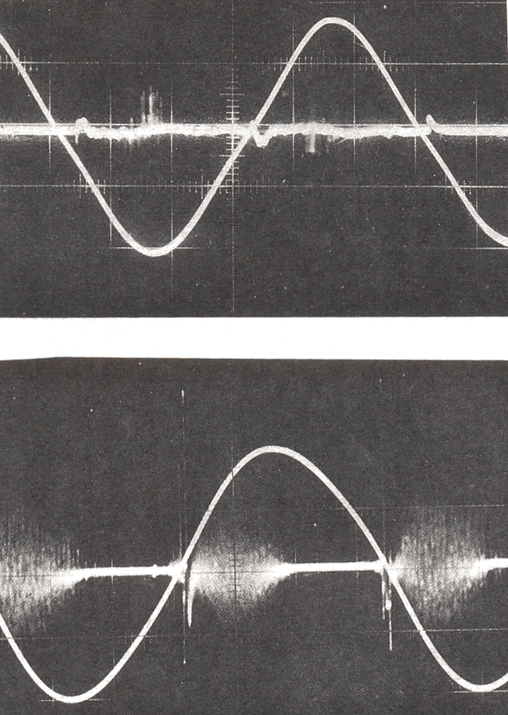
\includegraphics[width=\textwidth]{PartialDischargeWaveformDue}
    \caption{Partial Discharge Waveform Due to Voids in Insulating Material}
    \label{fig:Partial Discharge Waveform Due to Voids in Insulating Material}
\end{figure}

\clearpage 
Effect of Partial Discharge on Current Transformer
\begin{enumerate}


\item The phenomenon of partial discharge in high voltage current transformers will lead to the complete breakdown in the electrical network. The operation and performance will be deteriorated.

\item For study and analysis of partial discharge in current transformers, a Simulink model took for reference and effect due to partial discharges studied. The voids and insulation strength decided the partial discharge in oil filled current transformers. Also, the voltage level of current transformers will contribute to partial discharge.

\item From the Simulink model, different sizes of voids partial discharge pulses are studied and a number of PDs, magnitude, the frequency is calculated. This helps in knowing PD trend and further this data can be utilized to know the strength of insulation in high voltage current transformers.

\item The PD waveforms from Simulink model and calculated parameters used for oil and insulation papers sample, the characteristic of PDs has been studied.

\item The continuous Partial discharge in current transformers will reduce the insulation strength and will form the breakdown of electrical stress in the long term.

\item Partial discharge process leads to reduce insulation strength of insulating media oil and paper and will permanently damage the quality of insulation.

\item Partial discharge measurements are done to study effects caused due to PDs on insulation oil and can help in knowing the life of current transformers or actions for preventive maintenance \cite{gutfleisch1995measurement, bartnikas2002partial, karmakar2009partial}.

\end{enumerate}

\pagebreak 
\section{Motivation}
Detection and measure Partial Discharge Phenomenon in High Voltage Current Transformers ~145kV ~which ~is ~the ~main source ~of ~failure. The ~effect on the performance of insulation used in High Voltage Current Transformers 145kV during working conditions over the period of time with high stress needs to be studied in various conditions.\setlength{\parskip}{1em}

High voltage electrical instruments always have the problem of insulation failure because of insulation deterioration over the period of time. When the insulation fails, the electrical instrument gets damaged to the nonrecoverable status. Hence the study of Partial discharge in high voltage current transformers will help in understanding effects on insulations medium, preventive maintenance planning and healthy life of instruments. 

Application of High Voltage Current transformers is for measurement as CTPT unit and protection supply to relays in the circuit. The purpose of the current transformer is to step down current in the system to 5A or 1A which is measurable value \cite{karmakar2009monitoring}.

A current transformer is instrument transformer which reduces secondary current with reference to the ratios to the primary current. Thus it defined in terms of the ratio of primary to secondary current. As these transformers are used for measurement purpose accuracy is most important.

The variable flux in toroidal cores decides the current in the secondary of the current transformer. The secondary of the current transformer is defined in terms of turn ratio. The primary ampere turns helps in magnetizing the core and secondary current is induced \cite{kuffel2000high, kreuger1989partial, naiduhigh }.

The current transformers are designed considering current flowing in the primary circuit, accuracy, and ratios required, material of insulation and cargo material of cores.\\

Partial Discharge in High voltage Current Transformers is resulting in the breakdown of Instrument. A study needs to be done for analysis, reasons, and actions during the manufacturing process. Based on study improvements will be suggested to improve the performance of Product in Service. The breakdown will damage not only the Current transformer but also nearby Instruments in Sub Station. Hence study is required on Partial Discharges of Current Transformers which are going High Electrical Stress in working condition. The study is required for testing of Current Transformers  \cite{Proceedingsof2008International}.

During the manufacturing process, current transformers undergo various type test and routine test to meet the specifications at national and international level.

Some of the routine tests conducted on current transformers are\setlength{\parskip}{0em} 

\begin{enumerate}[label=\Roman*.]
\item Comparison test with standard CT, \textit{i.e.}, accuracy and phase error as per standard specifications

\item Insulation breakdown to know the strength of insulation by applying the high voltage to winding

\item Effect of temperature on the performance of insulation

\item Tan delta and insulation breakdown of oil

\item Short circuit current flowing capacity of insulating material
\end{enumerate}

\pagebreak 
\section{Objectives}
The objectives of this research work are to:
\begin{enumerate}
\item Propose Manufacturing Industries for Improvement in Performance of High Voltage Current Transformers

\item Study, Analyze and Measure Premature Failure of High Voltage Current Transformers

\item Provide actions in Manufacturing processes to minimize Partial Discharge phenomenon

\item Study On line and Off line Testing of Partial Discharge in High Voltage Current Transformers

\item Develop Mathematical Modeling of High Voltage Current Transformers

\item Simulate Model for High Voltage Current Transformers in Steady State Condition

\item Simulate Model for High Voltage Current Transformers in Short Circuit and Transient Condition
\end{enumerate}

\pagebreak 
\section{Theme}
The theme for this research work based on Partial Discharge Analysis of high voltage oil 
Filled current transformers 145 kV up to 3000 Amp used in high voltage Sub stations.
The study is concentrated on Improving the performance of Current Transformers hence
data from field and manufacturing process were conducted.\setlength{\parskip}{1em}
 
Having taken a due note of restraints upon efforts, resources and time, the study is
Confined mainly two areas, effect on Current Transformers during steady state Conditions
and during Short Circuit and Transient condition. Using MATLAB / Simulink model used
for comparative Study and the performance analysis carried out on the basis of various void
sizes developed and worked for effect of various void sizes on performance of Current 
Transformers. On the basis of results obtained improvement in existing manufacturing
process were suggested\setlength{\parskip}{0em}.

\begin{figure}[h!]
    \centering
    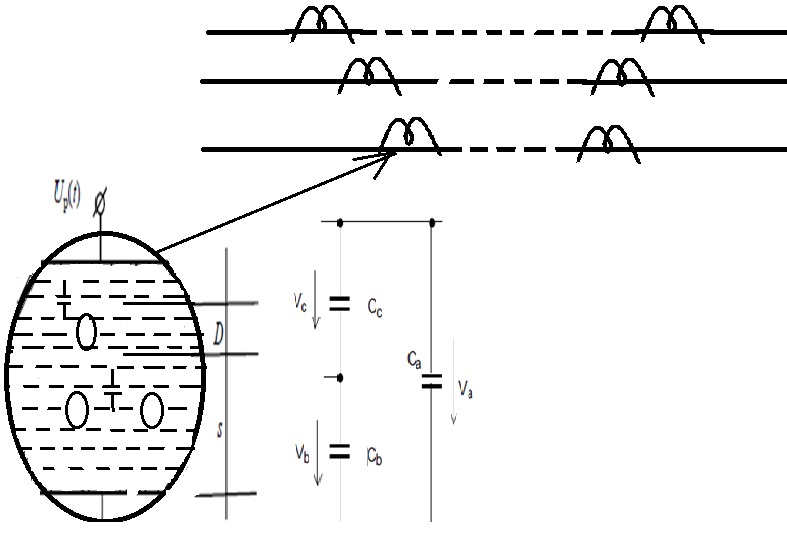
\includegraphics[width=\textwidth]{HighVoltageTransmissionLineWithCurrentTransformers}
    \caption{High Voltage Transmission Line With Current Transformers}
    \label{fig:High Voltage Transmission Line With Current Transformers}
\end{figure}

\pagebreak 
\section{Organization}
The ~research work titled \textquotedblleft Partial Discharge Analysis in High Voltage Filled Current Transformers 145 kV up to 3000 A\textquotedblright ~is organized in this Thesis among five chapters as per follow.\setlength{\parskip}{1em}

The first chapter gives Introduction of partial discharge phenomenon, and its effects on high voltage oil filled current transformers were given. The need and motivation for this research work mentioned and Objectives of this study work described. The Theme of the complete study work is presented.

A summary of the exhaustive literature survey is represented in second chapter. An overview of partial discharge and its effect on the performance of high Voltage electrical instruments in particular, oil filled current transformers were discussed in details.

Work done on System Development were discussed in third chapter. With the help of mathematical model of current Transformer and using MATLAB/SIMULINK software representing the steady state and Short circuit and transient conditions were run ~for different void sizes. Having taken ~various data ~from field ~and manufacturing process, need for developing Simulink model evolved to see the PD effect During Steady state, Short Circuit, and Transient Conditions. To attain Objectives of the study Manufacturing process of High Voltage Current Transformers were studied. Process Parameters, Insulation material, and strength, testing procedures, detection of Partial Discharge were studied. Analysis of these data was done and studied to meet Objectives. 

The Performance Analysis for the Simulink model mentioned in chapter 3 was done and explained in fourth chapter. Based on Collected data PD measurement were converted and Simulink model developed. The performance needs to be analyzed during steady state, Short Circuit and transients hence two Simulink models were developed. Data and PD were simulated with various kV applied and performance was interpreted and analyzed in the form of wave forms, strength and magnitude of partial discharge, number of partial discharges and its frequency of occurrence. PD pulses were observed for evaluation for different kV. This data was interpreted to find root causes of failures and problems to eliminate defects and effective corrective actions.

In the fifth chapter conclusion of the research work, future scope and the application of this research work are mentioned. 

To attain the above objectives and for getting information on Partial Discharge during ~Online ~performance of Current ~Transformers for ~145 kV ~survey ~was conducted of various Sub stations of 145 kV. Data of Various faults, failures, and analysis were conducted to get First-hand information on finding various information and to find reasons for Partial discharges.

As these High voltage current transformers and its electrical insulation undergo Various Thermal Stress, Chemical Attack and Abrasion due to excessive heat. From this model, PD Effect is studied for various kV voltages and different void sizes. Data collected for the number of PD, Frequency, Amplitude and predicted for PD effect. 

To Study, analyze performance High Voltage Current Transformers in field 145 kV Substations were selected. The performance in the field monitored during various conditions. Data collected for on line failures, its causes, various Measurements and its correlation with the performance of Current Transformers.

To Study the manufacturing process of High Voltage Current Transformers and collected data of various parameters which may lead to failures in Field. The Manufacturing process parameters such as High Vacuum level, Temperature, Oil low rate, Quality of Insulation material was studied and data collected. Acceptable limit of PD is between 5 pC to 10 pC. The Interpretation of data to Improve performance of PD were suggested.\setlength{\parskip}{0em}

%\setlength{\parskip}{1em}
%
%
%
%\begin{figure}[h!]
%    \centering
%    \includegraphics[width=\textwidth]{}
%    \caption{}
%    \label{fig:}
%\end{figure}
%
%
%
%\begin{table}[h!]
%\begin{threeparttable}
%\renewcommand{\arraystretch}{1.3}
%\caption{Percentage of Maf Rate and Mif Rate per Failure Mode, Third Inquiry.}
%\label{table:Percentage of Maf Rate}
%\centering
%\small
%\begin{tabular}{| >{\arraybackslash}m{1.9in} |>{\centering\arraybackslash}m{0.6in} |>{\arraybackslash}m{3in} |}
%
%%\begin{tabular}{| l | c | l |}
%\hline
%\multicolumn{1}{|c|}{\textbf{MaF failure mode}}	&	\textbf{MaF(\%)}	& \multicolumn{1}{|c|}{\textbf{Comments}}								\\ \hline
%Does not close on command	&	28.2				& Mainly with live tank circuit breakers			\\ \hline
%Does not open on command	&	16.4				&													\\ \hline
%Closes without command		&	0.2					&													\\ \hline
%Opens without command		&	5.4					&													\\ \hline
%Fails to carry the current	&	1.3					&													\\ \hline
%Dielectric breakdown		&9.9					& Breakdown to earth: 5\%, Internal breakdown across open pole, during opening operation = does not break the current: 1.9\%, Other across open pole: 1.8\%, Breakdown between poles: 1.2\%					\\ \hline
%Locked in open or closed position & 25.1			& Alarm has been triggered by the control system	\\ \hline
%Loss of mechanical integrity&	8.1					& Mechanical damage of parts						\\ \hline
%Other						&	5.2					&													\\ \hline
%Total						&	100					&													\\ \hline \hline
%\multicolumn{1}{|c|}{\textbf{MiF failure mode}}	& \textbf{Mif(\%)}		& \multicolumn{1}{|c|}{\textbf{Comments}}									\\ \hline
%Air or hydraulic oil leakage&	20.3				& In operating mechanism							\\ \hline
%Small SF\textsubscript{6} gas leakage		& 35.6					& Large leakage will give MF-mode \textquotedblleft
%Locked\textquotedblright
%			\\ \hline
%Oil leakage in grading capacitors &	1.0				&													\\ \hline
%Change in functional characteristics& 28.4			& 6.8\% mechanical; 3.3\% electrical 18.3\% control%
%													  and auxiliary systems								\\ \hline
%Other and no answer			& 14.6					&													\\ \hline
%Total						& 100					&													\\ \hline
%\end{tabular}
%%\begin{tablenotes}
%%\item \cmark -- functionality is available. \hspace{0.5in} \xmark -- functionality is not available.
%%\end{tablenotes}
%\end{threeparttable}
%\end{table}
%
%
%\section{Motivation}
%
%
%\clearpage
%\section{Objectives}
%
%
%\clearpage
%\section{Theme}
%
%\setlength{\parskip}{0em}
%\clearpage
%\section{Organization} 
%
%\subsubsection*{Chapter 1}